\section{Planificación y presupuesto}
En esta sección se detallará la organización y planificación del proyecto, 
así como el presupuesto necesario para llevarlo a cabo. Se utilizarán diagramas 
para facilitar la comprensión de los diferentes aspectos del proyecto.

\subsection{Plan de recursos humanos}
Uno de los activos más vitales en cualquier proyecto es 
el equipo humano. En este plan, se detallan las funciones y responsabilidades de 
cada miembro del equipo, con el fin de fomentar una colaboración efectiva y alcanzar 
los objetivos del proyecto. Entre los perfiles involucrados en el proyecto se
encuentran el director del proyecto, el director Tecnalia y el estudiante.

\begin{enumerate}
    \item \textbf{Director del proyecto}
    \begin{itemize}
        \item Descripción: El director del proyecto es a efectos prácticos el 
        encargado de supervisar que el proyecto siga la normativa de la universidad y la memoria sea correcta.
        Este perfil es ocupado por el tutor universitario asignado al proyecto.
        \item Responsabilidades:
        \begin{itemize}
            \item Supervisar que el proyecto cumpla con las normativas de la universidad.
            \item Validación del proyecto y trabajo del alumno.
            \item Supervisar las actividades del proyecto.
            \item Revisar y asegurar la corrección de la memoria del proyecto.
            \item Ayudar a que se cumplen los plazos establecidos por la universidad.
            \item Aportar horientación académica al estudiante.
        \end{itemize}
        \item Disponibilidad:
        \begin{itemize}
            \item Disponibilidad para realizar reuniones semanales de seguimiento. 
            \item Disponibilidad para resolver dudas via correo electrónico.
        \end{itemize}
    \end{itemize}
    
    \item \textbf{Director Tecnalia}
    \begin{itemize}
        \item Descripción: El director Tecnalia es el encargado de supervisar que el 
        proyecto se alinee con las necesidades de la empresa y aportar su experiencia 
        en el desarrollo de sistemas de IA. En este perfil se incluyen dos directores,
        uno de ellos enfocado en el desarrollo del sistema y otro en la parte de pruebas
        y validación.
        \item Responsabilidades:
        \begin{itemize}
            \item Recolección de requisitos y definición de objetivos.
            \item Asegurar que el desarrollo del proyecto se alinee con las necesidades de la empresa.
            \item Proporcionar apoyo en la investigación.
            \item Supervisar las actividades del proyecto.
            \item Ofrecer feedback constante sobre el desarrollo del proyecto.
            \item Ayudar al estudiante proporcionándole recursos para las pruebas del sistema.
        \end{itemize}
        \item Disponibilidad:
        \begin{itemize}
            \item Horario laboral estándar, con flexibilidad para reuniones con el estudiante.
            \item Disponibilidad para resolver dudas via correo electrónico.
        \end{itemize}
    \end{itemize}

    \item \textbf{Estudiante}
    \begin{itemize}
        \item Descripción: El director del proyecto es a efectos prácticos el 
        encargado de supervisar que el proyecto siga la normativa de la universidad y la memoria sea correcta.
        Este perfil es ocupado por el tutor universitario asignado al proyecto.
        \item Responsabilidades:
        \begin{itemize}
            \item Desarrollar el proyecto bajo la orientación de los tutores.
            \item Redactar la memoria del proyecto.
            \item Realizar pruebas del sistema.
            \item Presentar avances periódicos al equipo de tutores.
        \end{itemize}
        \item Disponibilidad:
        \begin{itemize}
            \item Horario laboral estándar, con flexibilidad para reuniones con el estudiante.
        \end{itemize}
    \end{itemize}
\end{enumerate}

\subsection{Programa de trabajo}
La siguiente sección detallará el plan de trabajo seguido en el proyecto,
incluyendo las diferentes tareas generales realizadas con su duración planificada y real,
junto con el diagrama de Gantt del proyecto. Las tareas del proyecto se han
dividido en tres fases distintas. La primera fase incluye las tareas necesarias
para el desarrollo del MVP del proyecto, que incluye la creación de un sistema
funcional y su respectiva presentación al equipo de trabajo. La segunda fase 
incluye la implementación de las diferentes diferentes plataformas y automatizaciones
necesarias para garantizar la seguridad y escalabilidad del sistema. La tercera
fase se basa en probar el sistema con diferentes problemas de series temporales y
recaudar información sobre los resultados, contenido relevante para el sistema de
conocimiento y la documentación final del proyecto.

\subsubsection{Fase 1: Desarrollo del MVP}
Esta fase está formada por una serie de tareas que se deben completar para
la creación del producto mínimo viable. Las tareas incluidas en esta fase son
aquellas indispensable para realizar una prueba de concepto y valorar la viabilidad
técnica del proyecto. Las tareas incluidas en esta fase son las siguientes:

\begin{itemize}
    \item \textbf{Tarea 1.1:} Investigación inicial sobre el estado del arte,
    tecnologías y herramientas necesarias para el proyecto.
    \item \textbf{Tarea 1.2:} Definición del alcance del MVP y la hoja de ruta
    para su desarrollo.
    \item \textbf{Tarea 1.3:} Definición del plan de trabajo y el como debe
    ser utilizada la herramienta.
    \item \textbf{Tarea 1.4:} Desarrollo del sistema de componentes y plantillas.
    \item \textbf{Tarea 1.5:} Despliegue básico de ClearMl y configuración de
    \item \textbf{Tarea 1.6:} Implantación de empaquetado automático de los
    paquetes y subida a un repositorio de artefactos.
    los experimentos.
    \item \textbf{Tarea 1.7:} Presentación del MVP y validación de la viabilidad.
\end{itemize}

\subsubsection{Fase 2: Integración de nuevas plataformas, securizacion y despliegue}
Esta fase está formada por una serie de tareas que incluyen la implementación
de las diferentes partes del proyecto. Las tareas incluidas en esta fase son
las siguientes:

\begin{itemize}
    \item \textbf{Tarea 2.1:} Integración de nuevas plataformas para la
    visualización de los experimentos.
    \item \textbf{Tarea 2.2:} Securización de la infraestructura utilizando
    un proxy inverso con Nginx y Keycloak.
    \item \textbf{Tarea 2.3:} Despliegue de la infraestructura de forma automática
    utilizando GitLab CI/CD.
    \item \textbf{Tarea 2.4:} Automatización de la creación de componentes y
    plantillas proporcionando una plantilla base para cada caso.
    \item \textbf{Tarea 2.5:} Creación de la documentación técnica y de usuario.
    \item \textbf{Tarea 2.6:} Lanzamiento de pruebas unitarias de los componentes.
\end{itemize}

\subsubsection{Fase 3: Experimentación, pruebas y documentación}
El último bloque de tareas incluye la experimentación, el análisis de los
resultados obtenidos y la documentación final del proyecto. Esta ultima es
fundamental debido a que el proyecto se desarrolla en un entorno de
investigación y es necesario documentar todo el procedimiento para que puede
ser aplicado por otros investigadores. Las tareas incluidas en esta fase son
las siguientes:

\begin{itemize}
    \item \textbf{Tarea 3.1:} Prueba del sistema para un problema de forecasting.
    \item \textbf{Tarea 3.2:} Prueba del sistema para un problema de clasificación.
    \item \textbf{Tarea 3.3:} Prueba del sistema para un problema de detection de anomalías.
    \item \textbf{Tarea 3.4:} Implantación del sistema en el entorno de trabajo del equipo.
    \item \textbf{Tarea 3.5:} Encuesta de satisfacción y feedback de los resultados.
    \item \textbf{Tarea 3.6:} Redacción de la memoria del proyecto.
\end{itemize}

\subsubsection{Diagrama de Gantt}
A continuación se muestra el diagrama de Gantt del proyecto, donde se puede
observar la planificación temporal de las diferentes tareas descritas
anteriormente. El proyecto al estar dividido en tres fases se ha utilizado el
color azul para representar la fase 1, el color verde para la fase 2 y el color
morado para la fase 3. Se ha respetado cuidadosamente el tiempo de cada tarea y
el proyecto no ha sufrido ningún retraso durante su desarrollo.

\begin{figure}
    \centering
    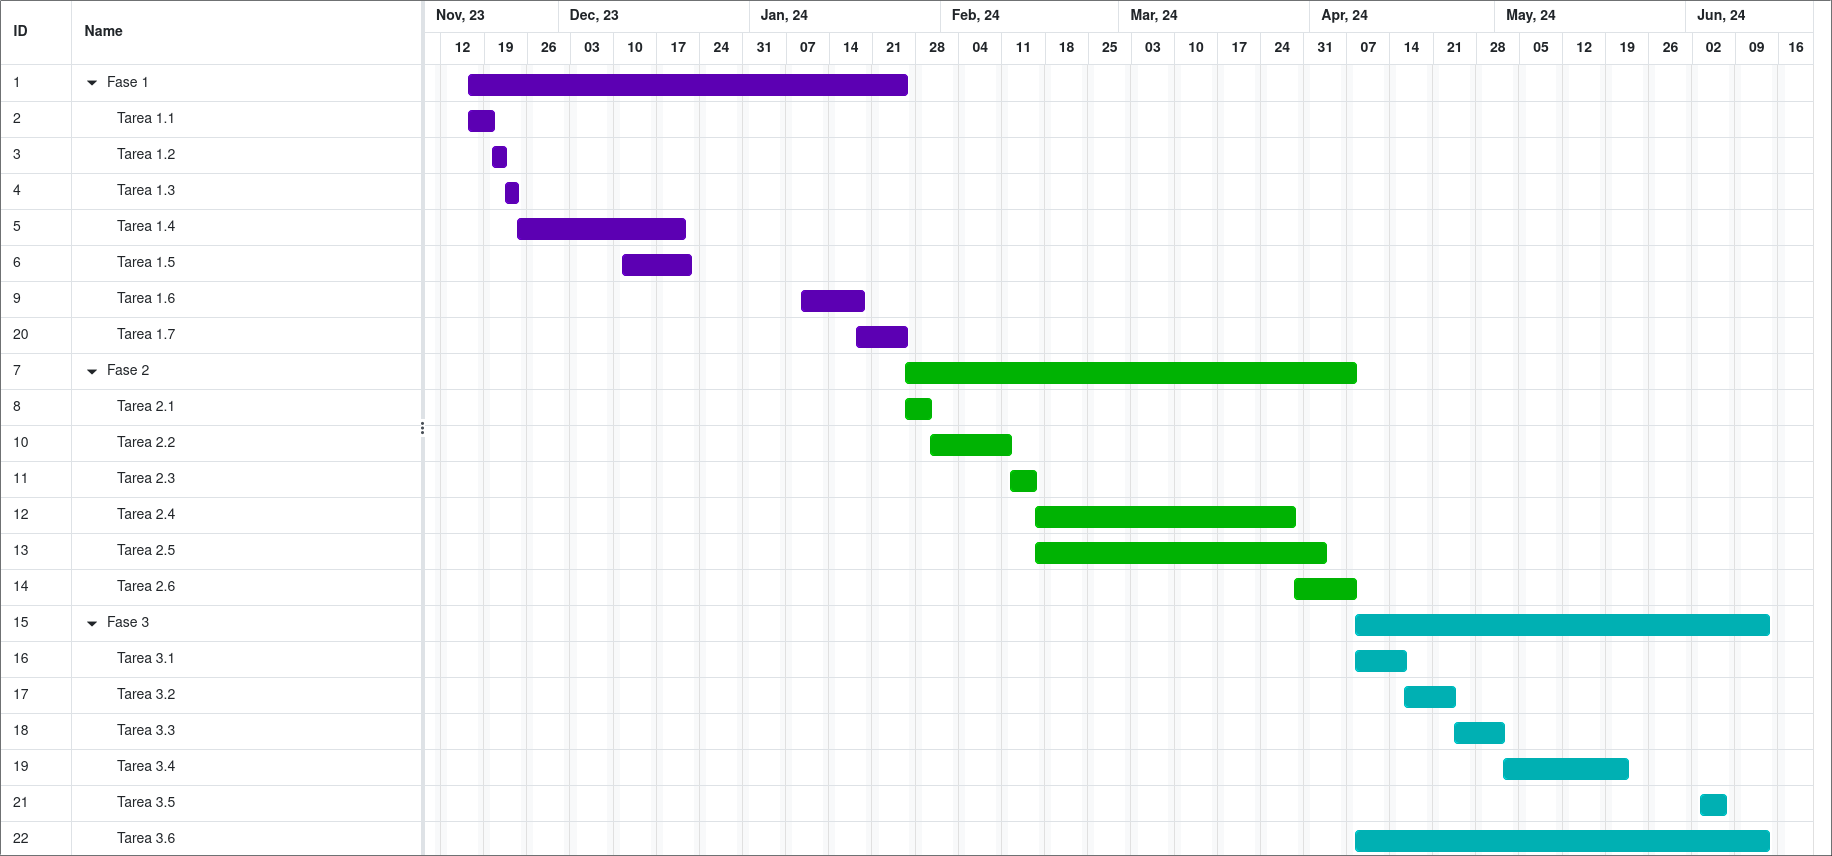
\includegraphics[angle=90, width=\textwidth, height=\textheight, keepaspectratio]{gantt.png}
    \caption{Diagrama de planificación del proyecto.}
    \label{fig:gantt-planification}
\end{figure}

\pagebreak
\subsection{Tabla de tareas}
\begin{table}[ht]
    \centering
    \begin{tabular}{|c|c|c|c|c|}
    \hline
    \textbf{Fase/Tarea} & \textbf{Fecha inicio} & \textbf{Fecha fin} & \textbf{Duración} \\
    \hline
    \textbf{Fase 1} & Noviembre 22, 2023 & Enero 26, 2024 & 52 días \\
    \hline
    T1.1 & Noviembre 22, 2023 & Noviembre 24, 2023 & 03 días \\
    T1.2 & Noviembre 24, 2023 & Diciembre 21, 2023 & 20 días \\
    T1.3 & Diciembre 11, 2023 & Diciembre 22, 2023 & 10 días \\
    T1.4 & Enero 09, 2024 & Enero 19, 2024 & 09 días \\
    T1.5 & Enero 18, 2024 & Enero 26, 2024 & 07 días \\
    \hline
    \textbf{Fase 2} & Enero 26, 2024 & Abril 08, 2024 & 52 días \\
    \hline
    T2.1 & Enero 26, 2024 & Enero 30, 2024 & 03 días \\
    T2.2 & Enero 30, 2024 & Febrero 12, 2024 & 10 días \\
    T2.3 & Febrero 12, 2024 & Febrero 16, 2024 & 05 días \\
    T2.4 & Febrero 16, 2024 & Marzo 29, 2024 & 31 días \\
    T2.5 & Febrero 16, 2024 & Abril 03, 2024 & 34 días \\
    T2.6 & Marzo 29, 2024 & Abril 08, 2024 & 07 días \\
    \hline
    \textbf{Fase 3} & Abril 08, 2024 & Junio 14, 2024 & 50 días \\
    \hline
    T3.1 & Abril 08, 2024 & Abril 16, 2024 & 07 días \\
    T3.2 & Abril 16, 2024 & Abril 24, 2024 & 07 días \\
    T3.3 & Abril 24, 2024 & Mayo 02, 2024 & 07 días \\
    T3.4 & Mayo 02, 2024 & Mayo 22, 2024 & 15 días \\
    T3.5 & Junio 03, 2024 & Junio 07, 2024 & 05 días \\
    T3.6 & Abril 08, 2024 & Junio 14, 2024 & 45 días \\
    \hline
    \end{tabular}
    \caption{Resumen de las tareas y fases}
    \label{tab:my_label}
    \end{table}

\subsection{Presupuesto}
La siguiente sección detallará el presupuesto necesario para llevar a cabo el
proyecto, incluyendo los diferentes recursos necesarios y su coste. El
presupuesto se ha dividido en tres categorías principales: recursos humanos,
hardware y software.

\subsubsection{Recursos humanos}
La siguiente tabla muestra el coste de los diferentes perfiles involucrados en
el proyecto, así como el número de horas invertidas por cada uno de ellos y el
coste total de cada perfil.

\begin{table}[ht]
    \centering
    \begin{tabular}[ht]{l|c|c|c}
        \textbf{Perfil}       & \textbf{Coste por Unidad} & \textbf{Horas Invertidas} & \textbf{Precio Total} \\
        \hline
        Director del proyecto & 40\euro/h             & 20h                       & 800\euro              \\
        Director Tecnalia 1   & 90\euro/h             & 60h                       & 5.400\euro            \\
        Director Tecnalia 2   & 90\euro/h             & 20h                       & 1.800\euro            \\
        Estudiante            & 6.5\euro/h            & 540h                      & 3.500\euro            \\
        \hline
        Total                 & 17.95\euro/h           & 640h                      & 11.500\euro           \\
    \end{tabular}
    \caption{Presupuesto de recursos humanos}\label{tab:huma-resources}
\end{table}

\subsubsection{Hardware}
La siguiente tabla muestra el coste de los diferentes recursos hardware
necesarios para llevar a cabo el proyecto, así como el número de unidades
necesarias y el coste total de cada recurso.

\begin{table}[ht]
    \centering
    \begin{tabular}[ht]{l|c|c|c}
        \textbf{Recurso}     & \textbf{Coste por unidad} & \textbf{Unidades} & \textbf{Precio Total} \\
        \hline
        Hora máquina virtual & 0.2\euro                  & 200u              & 40\euro               \\
        Portátil             & 700\euro                  & 1u                & 700\euro              \\
    \end{tabular}
    \caption{Presupuesto hardware}
    \label{tab:hardware-budget}
\end{table}

\subsubsection{Software}
Los recursos software necesarios para llevar a cabo el proyecto son gratuitos
en su mayoría, a excepción de la licencia de GitHub Copilot que tiene un coste
de 10\euro/mes. Aun así, se ha utilizado la versión gratuita que viene incluida
con la licencia de GitHub Pro por ser estudiante.

\subsubsection{Mantenimiento Futuro}
La siguiente sección estima el coste de mantener el sistema durante un año, teniendo 
en cuenta los recursos humanos, hardware y software necesarios para su operación continua.
Para este caso se ha considerado dos perfiles de recursos humanos, un desarrollador MLOPs
y un director de proyecto. 

\begin{table}[h]
    \centering
    \begin{tabular}[H]{l|c|c|c|c}
        \textbf{Recurso}           & \textbf{Coste Unidad} & \textbf{Cantidad} & \textbf{Frecuencia} & \textbf{Precio Total Anual} \\
        \hline
        Director de Proyecto        & 90\euro/h             & 2h/mes            & 12 meses           & 2.160\euro \\
        Desarrollador MLOPs         & 90\euro/h             & 10h/mes           & 12 meses           & 10.800\euro \\
        Servidor de produccion       & 0.2\euro              & 720h/mes         & 12 meses           & 1.728\euro   \\
        Servidor de desarrollo       & 0.1\euro              & 15h/mes          & 12 meses           & 432\euro   \\
        \hline
        \multicolumn{4}{r|}{Total Anual} & 15.111\euro \\
    \end{tabular}
    \caption{Presupuesto futuro anual para el mantenimiento del sistema}
    \label{tab:future-budget}
\end{table}

\subsubsection{Total}
A continuación se muestra el presupuesto general del proyecto, incluyendo el
coste total de los recursos humanos, hardware y software necesarios para llevar
a cabo el desarrollo.

\begin{table}
    \centering
    \begin{tabular}[H]{l|r}
        \textbf{Recurso} & \textbf{Precio Total} \\
        \hline
        Recursos humanos & 11.500\euro           \\
        Hardware         & 740\euro              \\
        Software         & 0\euro                \\
        \hline
        Total            & 12.240\euro           \\
    \end{tabular}
    \caption{Presupuesto general}
    \label{tab:total-budget}
\end{table}

\break


\pagebreak